\lecture{17}{3. November 2025}{Fluid Flows About Immersed Bodies -- Drag, Lift and Airfoils}

Whenever a body moves relatively to a viscous fluid surrounding it, the body will experience a net force $\Vec{F}$.
The magnitude of this force depends on factors such as relative velocity $\Vec{V}$, body shape, body size, fluid properties and so forth.
As the fluid flows around the immersed body, it will generate surface stresses on each element of the surface, resulting in the aforementioned force.
The surface stresses are composed of a tangential component due to viscous action and a normal component due to pressure action.

\subsection{Drag}
Drag is the component of force on a body acting parallel to the direction of relative motion (i.e. left/right for a 1 dimensional body moving left to right). 
In \Cref{eq:dragsym} a functional form of the drag force $F_D$ was given as
\[ 
F_D = f_1 (d, V, \mu, \rho)
.\]
Application of the Buckingham Pi theorem resulted in two dimensionless $\Pi$ parameters that were written in functional form as
\[ 
\frac{F_D}{\rho V^2 d^2} = f_2 \left( \frac{\rho V d}{\mu} \right) = f_2 \left( \mathrm{Re} \right)
.\]
As $d^2$ is proportional to cross sectional area we could also write
\begin{equation} \label{eq:dragdim}
  \frac{F_D}{\rho V^2 A} = f_3 \left( \frac{\rho V d}{\mu} \right) = f_3 \left( \mathrm{Re} \right)
\end{equation}
This is valid for incompressible flow over \textit{any} body.

The \textit{drag coefficient}, $C_D$, is defined as
\begin{equation*}
  C_D \equiv \frac{F_D}{\frac{1}{2}\rho V^2 A}
.\end{equation*}

Using this \Cref{eq:dragdim} can be written as
\begin{equation*}
  C_D = f(\mathrm{Re})
.\end{equation*}

If compressibility and free-surface effects are also included in this the following functional form is obtained instead
\begin{equation*}
  C_D = f(\mathrm{Re}, \mathrm{Fr}, M)
.\end{equation*}


\subsubsection{Pure Friction Drag: Flow over a Flat Plate Parallel to the Flow}
This is the same flow situation as was discussed in \Cref{sec:flatplate}.
Since the pressure gradient is zero and pressure forces that are perpendicular to the plate do not contribute to the drag, the total drag is equal to the friction drag.
This
\begin{equation*}
  F_D = \int_{\text{plate surface}} \tau_w \, \mathrm{d}A
\end{equation*}
and
\begin{equation} \label{eq:dragflatplate}
  C_D = \frac{F_D}{\frac{1}{2}\rho V^2 A} = \frac{\int_{\mathrm{PS}} \tau_w \, \mathrm{d}A}{\frac{1}{2} \rho V^2 A}
\end{equation}
where $A$ is the total surface area in contact with the fluid.
The drag coefficient for a flat plate parallel to the flow depends on the shear stress distribution along the plate.

For laminar flow over a flat plate, the shear stress coefficient was, in \Cref{eq:shearstressflatplate} given as
\begin{equation*}
  C_f = \frac{\tau_w}{\frac{1}{2}\rho U^2} = \frac{\num{0,664} }{\sqrt{\mathrm{Re}_x}}
.\end{equation*}
The drag coefficient $C_D$ for flow with free stream velocity $V$, over a flat plate of length $L$ and width $b$ is then obtained by substituting $\tau_w$ from \Cref{eq:shearstressflatplate} into \Cref{eq:dragflatplate} as
\begin{align*}
    C_D &= \frac{1}{A} \int_{A} \num{0,664} \mathrm{Re}_x^{-\num{0,5} } \, \mathrm{d}A \\
    &= \frac{1}{bL} \int_{0}^{L} \num{0,664} \left( \frac{V}{\nu} \right)^{- \num{0,5} } x^{-\num{0,5} } b \, \mathrm{d}x  \\
    &= \frac{\num{0,664} }{L} \left( \frac{\nu}{V} \right)^{\num{0,5} } \left[ \frac{x^{\num{0,5} }}{\num{0,5} } \right]_{0}^{L} \\
    &= \num{1,33} \left( \frac{\nu}{VL} \right)^{\num{0,5} } \\
    &= \frac{\num{1,33} }{\sqrt{\mathrm{Re}_L}}
.\end{align*}

Assuming the boundary layer is turbulent from the leading edge, the shear stress coefficient, as given by the numerical results from \Cref{fig:f9_4}, is given by
\begin{equation} \label{eq:shearstressflatplateturb}
  C_f = \frac{\tau_w}{\frac{1}{2}\rho U^2} = \frac{\num{0,0594} }{\mathrm{Re}_x^{\frac{1}{5}}}
.\end{equation}
Substituting $\tau_w$ from \Cref{eq:shearstressflatplateturb} into \Cref{eq:dragflatplate} we get
\begin{align*}
  C_D &= \frac{1}{A} \int_A \num{0,0594} \mathrm{Re}_x^{-\num{0,2} } \, \mathrm{d}A \\
  &= \frac{1}{bL} \int_{0}^{L} \num{0,0594} \left( \frac{V}{\nu} \right)^{-\num{0,2} }x^{-\num{0,2} }b \, \mathrm{d}x  \\
  &= \frac{\num{0,0594} }{L} \left( \frac{\nu}{V} \right)^{\num{0,2} } \left[ \frac{x^{\num{0,8} }}{\num{0,8} } \right]_{0}^{L} \\
  &= \num{0,0742}  \left( \frac{\nu}{VL} \right)^{\num{0,2} } \\
  &= \frac{\num{0,0742}}{\mathrm{Re}_L^{\frac{1}{5}}}
.\end{align*}
The above result is valid for $\num{5e5} < \mathrm{Re}_L < \num{e7}$.

For $Re_L < \num{e9}$ an empirical result has been found to be
\begin{equation*}
  C_D = \frac{\num{0,455} }{\left( \log \mathrm{Re}_L \right)^{\num{2,58}}}
.\end{equation*}

For a boundary layer that is initially laminar and undergoes transition at some location on the plate, the turbulent drag coefficient must be adjusted to account for laminar flow over the initial length.
This adjustment is made by subtracting $B / \mathrm{Re}_L$ from the $C_D$ determined for completely turbulent flow.
The value of $B$ depends on the Reynolds number at transition, as
\begin{equation*}
  B = \mathrm{Re}_{\mathrm{tr}} \left( C_{D_{\text{turbulent}}} - C_{D_{\text{laminar}}} \right)
.\end{equation*}
For a transition Reynolds number of \num{5e5}, the drag coefficient may be calculated by adjusting either of the formulae for the turbulent drag coefficients as:
\begin{align*}
  C_D &= \frac{\num{0,0742}}{\mathrm{Re}_L^{\frac{1}{5}}} - \frac{\num{1740} }{\mathrm{Re}_L} & \bigg( \num{5e5} &< \mathrm{Re}_L < \num{e7}  \bigg) \\
  C_D &= \frac{\num{0,455} }{\left( \log \mathrm{Re}_L \right)^{\num{2,58} }} - \frac{\num{1610} }{\mathrm{Re}_L} & \bigg( \num{5e5}  &< \mathrm{Re}_L < \num{e7} \bigg)
.\end{align*}

The variation of the drag coefficient for a flat plate parallel to the flow is shown on \Cref{fig:f9_8}.
On \Cref{fig:f9_8}, transition was assumed to occur at $\mathrm{Re}_x = \num{5e5}$ for flows in which the boundary layer was initially laminar.
The actual Reynolds number for which this transition happens depends on a variety of factors such as surface roughness, disturbances, etc. 

\begin{figure} [ht]
  \centering
  
\includegraphics[width=0.8\linewidth]{./figures/f9_8.png}
  \caption{Variation of drag coefficient with Reynolds number for a smooth flat plate parallel to the flow.}
  \label{fig:f9_8}
\end{figure}

\subsubsection{Pure Pressure Drag: Flow over a Flat Plate Normal to the Flow}
In flow over a flat plate normal to the flow, as shown on \Cref{fig:f9_9}, the wall shear stress is perpendicular to the flow direction and therefore does not contribute to the drag force.
The drag is given by
\begin{equation*}
  F_D = \int_{\text{surface}} \rho \, \mathrm{d}A
.\end{equation*}

For this geometry, the flow separates from the edges of the plate; i.e. there is a back-flow in the low energy wake of the plate.
This means that although the pressure at the rear surface of the plate is essentially constant, its magnitude cannot be determined analytically.
Therefore, we must resort to experiments to determine the drag force.

\begin{figure} [ht]
  \centering
  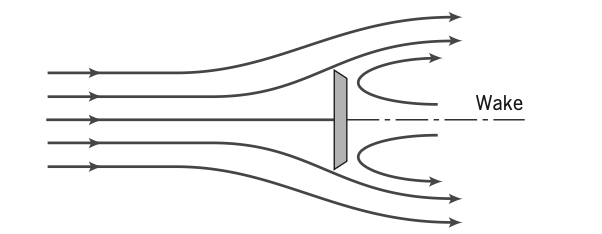
\includegraphics[width=0.5\linewidth]{./figures/f9_9.png}
  \caption{Flow over a flat plate normal to the flow}
  \label{fig:f9_9}
\end{figure}

The drag coefficient for flow over an immersed object is usually based on the frontal area of the object.
The drag coefficient for a finite plate normal to the flow depends on the ratio of plate width to height and on the Reynolds number.
For $\mathrm{Re}$ (based on height) greater than about \num{1000}, the drag coefficient is essentially independent of the Reynolds number.
The variation of $C_D$ with the ratio of plate width to height $b / h$ is shown on \Cref{fig:f9_10}.
For $b / h = \num{1,0} $ the drag coefficient is a minimum at $C_D = \num{1,18}$, which is just slightly higher than for a circular disk with $C_D = \num{1,17} $ at large Reynolds number.

For objects with sharp edges, the drag coefficient is essentially independent of Reynolds number (for $Re \geq \num{1000}$).
On \Cref{fig:dragco} drag coefficients for selected objects for $\mathrm{Re} \geq \num{e3}$ is shown.

\begin{figure} [ht]
  \centering
  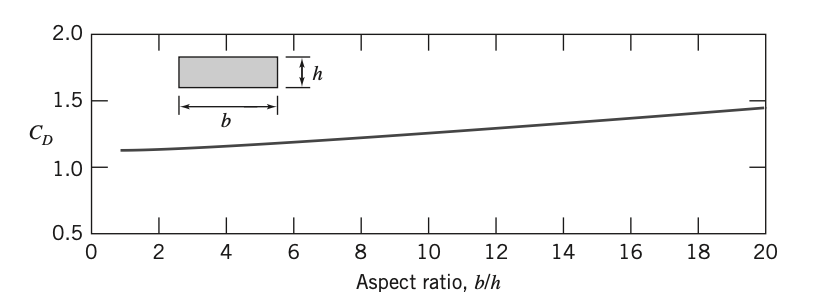
\includegraphics[width=0.7\linewidth]{./figures/f9_10.png}
  \caption{Variation of drag coefficient with aspect ratio for a flat finite plate normal to the flow with $\mathrm{Re}_h > \num{1000}$.}
  \label{fig:f9_10}
\end{figure}

\begin{figure} [ht]
  \centering
  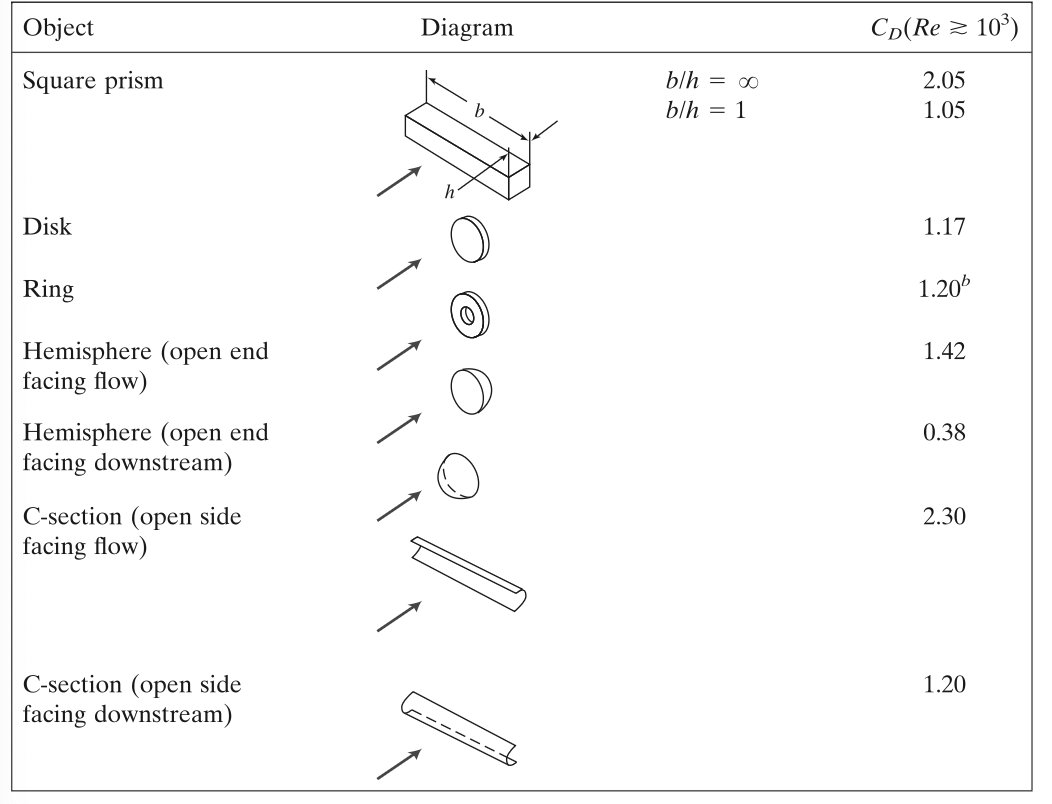
\includegraphics[width=0.6\linewidth]{./figures/dragco.png}
  \caption{Drag Coefficient Data for Selected Objects for $\mathrm{Re} \geq \num{e3} $}
  \label{fig:dragco}
\end{figure}

\subsubsection{Friction and Pressure Drag: Flow over a Sphere and Cylinder}
We have looked at two special flow cases, in which either friction or pressure drag was the sole form of drag present.
For friction-dominated drag, the drag coefficient was highly dependent on Reynolds number and for pressure-dominated drag the drag coefficient was largely independent of Reynolds number for $\mathrm{Re} \geq \num{1000}$.

For flow over a sphere, both friction and pressure drag contribute noteworthily to the total drag.
The drag coefficient for flow over a smooth sphere as a function of Reynolds number is depicted on \Cref{fig:f9_11}.

\begin{figure} [ht]
  \centering
  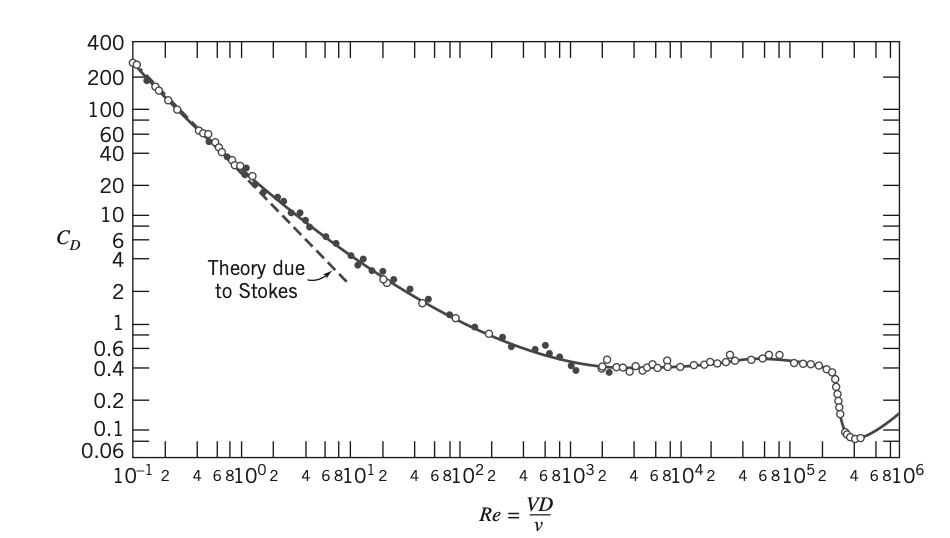
\includegraphics[width=0.8\linewidth]{./figures/f9_11.png}
  \caption{Drag coefficient of a smooth sphere as a function of Reynolds number.}
  \label{fig:f9_11}
\end{figure}

At very low Reynolds number, $\mathrm{Re} \leq 1$, there is no flow separation from a sphere; i.e. the wake is laminar and friction-drag will therefore dominate.
For very low Reynolds number flows, where inertia forces may be neglected, the drag force on a sphere of diameter $d$, moving at speed $V$ through a fluid of viscosity $\mu$ is
\begin{equation*}
  F_D = 3 \mu \pi V d
.\end{equation*}
The drag coefficient, $C_D$ is then
\begin{equation*}
  C_D = \frac{24}{\mathrm{Re}}
.\end{equation*}

As shown on \Cref{fig:f9_11} this expression agrees with experimental values at low Reynolds numbers, but it begins to deviate significantly from the data for $\mathrm{Re} > \num{1,0} $.

As the Reynolds number increases further, the drag coefficient drops up to a Reynolds number of about \num{1000}.
A turbulent wake develops and grows as the separation point moves from the rear of the sphere toward the front.
This wake leads to a relatively large amount of pressure drag.
At $\mathrm{Re} \approx \num{1000}$, about 95\% of the total drag is due to pressure.
For $\num{e3}  < \mathrm{Re} < \num{3e5} $, the drag coefficient is approximately constant.
In this range the entire sphere has a low-pressure turbulent wake, as indicated on \Cref{fig:f9_12}.
Note that $C_D \propto 1 / \mathrm{Re}$ corresponds to $F_D \propto V$, and that $C_D \sim \mathrm{constant}$ corresponds to $F_D \propto V^2$, indicating a rapid increase in drag.

\begin{figure} [ht]
  \centering
  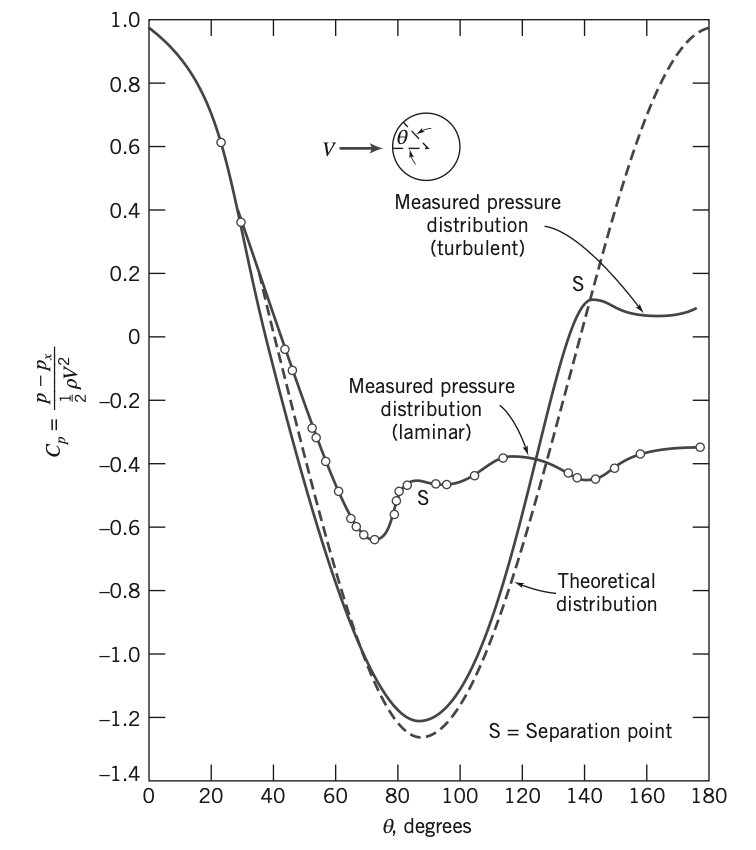
\includegraphics[width=0.5\linewidth]{./figures/f9_12.png}
  \caption{Pressure distribution around a smooth sphere for laminar and turbulent boundary-layer flow, compared with inviscid flow.}
  \label{fig:f9_12}
\end{figure}

For Reynolds numbers larger than about \num{3e5}, transition occurs and the boundary on the forward portion of the sphere becomes turbulent, which in turn leads to a decrease in the size of the wake, leading to an abrupt decrease in drag coefficient.

A turbulent boundary layer can, due to its higher momentum flux, better resist an adverse pressure gradient.
Consequently, a turbulent boundary-layer is desirable on a blunt body as it delays separation and in turn reduces pressure drag.

The drag coefficient for a sphere with a turbulent boundary layer is about $1 / 5$ that for laminar flow near the critical Reynolds number.
This is the reason golf balls are equipped with dimples.


\subsection{Lift}
For most objects in motion through a fluid the most significant force is drag.
However for some objects, such as airfoils, lift effects are also significant.
Lift is defined as the component of fluid force perpendicular to the fluid motion.
For an airfoil, the lift coefficient, $C_L$, is defined as
\begin{equation*}
  C_L \equiv \frac{F_L}{\frac{1}{2}\rho V^2 A_p}
.\end{equation*}

The lift and drag coefficients for an airfoil are functions of both Reynolds number and angle of attack (AoA).
The AoA, $\alpha$, is the angle between the airfoil chord and the free stream velocity vector.
The \textit{chord} of an airfoil is the straight line joining its leading and trailing edges.

Airfoil stall results when flow separation occurs over a major portion of the upper surface of the airfoil.
As the AoA is increased, the stagnation point moves back along the lower surface of the airfoil as shown schematically for the symmetric laminar-flow section on \Cref{fig:f9_18a}.
Flow on the upper surface must then accelerate sharply to round the nose of the airfoil.
The effect of AoA on the theoretical upper surface pressure distribution is shown on \Cref{fig:f9_18b}.
The minimum pressure becomes lower, and its location moves forward on the upper surface. 
A severe pressure gradient will appear following the point of minimum pressure, which causes the flow to separate completely from the upper surface and the airfoil stalls.

\begin{figure} [ht]
  \centering
  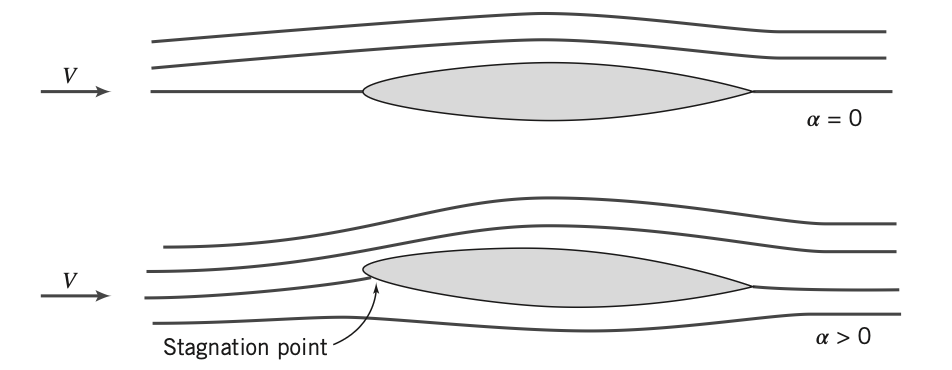
\includegraphics[width=0.7\linewidth]{./figures/f9_18a.png}
  \caption{Effects of angle of attack on flow pattern.}
  \label{fig:f9_18a}
\end{figure}

\begin{figure} [ht]
  \centering
  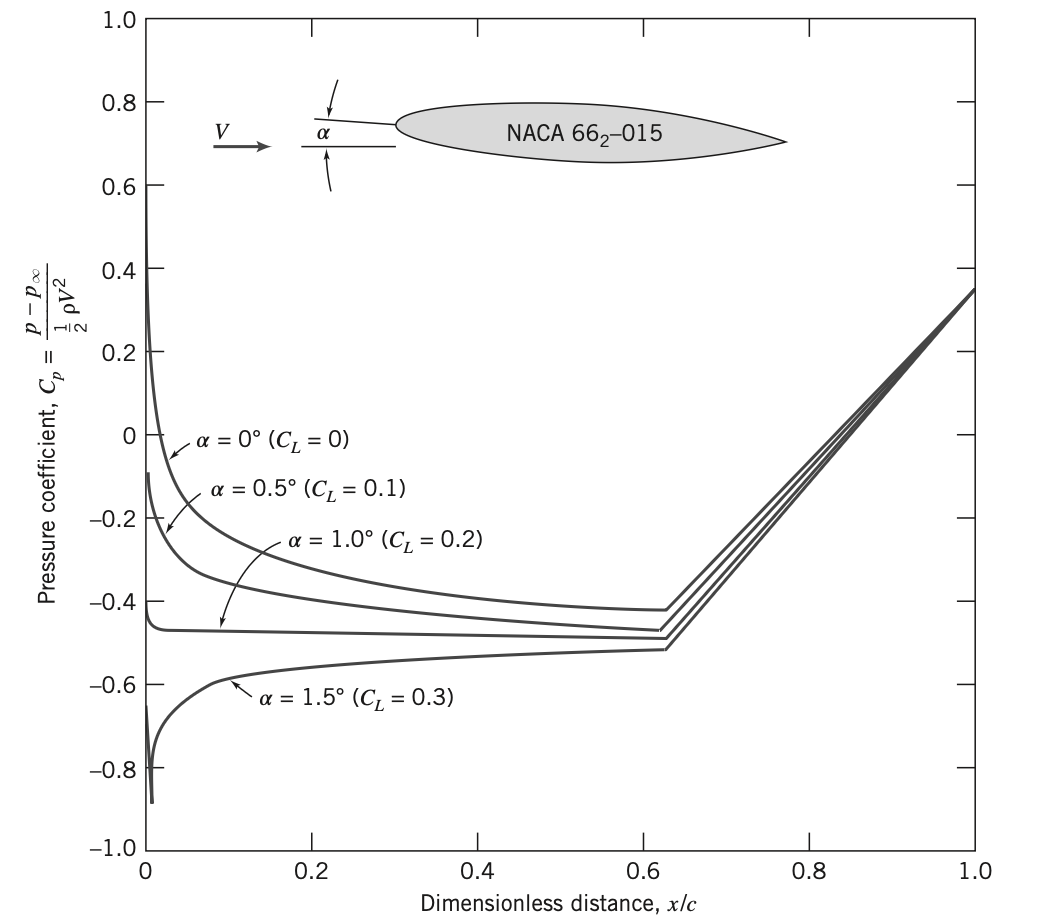
\includegraphics[width=0.7\linewidth]{./figures/f9_18b.png}
  \caption{Effect of angle of attack on theoretical pressure distribution for a symmetric laminar flow airfoil of 15\% thickness ratio.}
  \label{fig:f9_18b}
\end{figure}

Stall is indicated on \Cref{fig:f9_17a} as the AoA for which the lift coefficient decreases sharply.

\begin{figure} [ht]
  \centering
  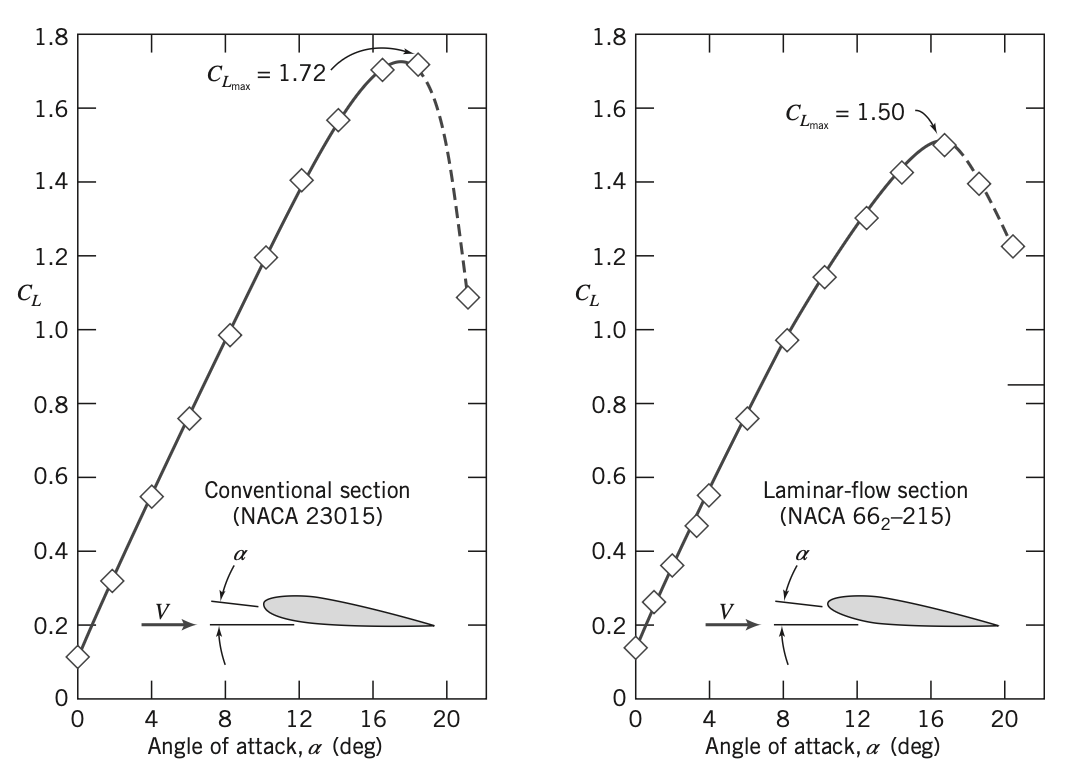
\includegraphics[width=0.6\linewidth]{./figures/f9_17a.png}
  \caption{Lift coefficient versus angle of attack for two airfoil sections of 15\% thickness ratio at $\mathrm{Re}_c = \num{9e6} $.}
  \label{fig:f9_17a}
\end{figure}

\begin{figure} [ht]
  \centering
  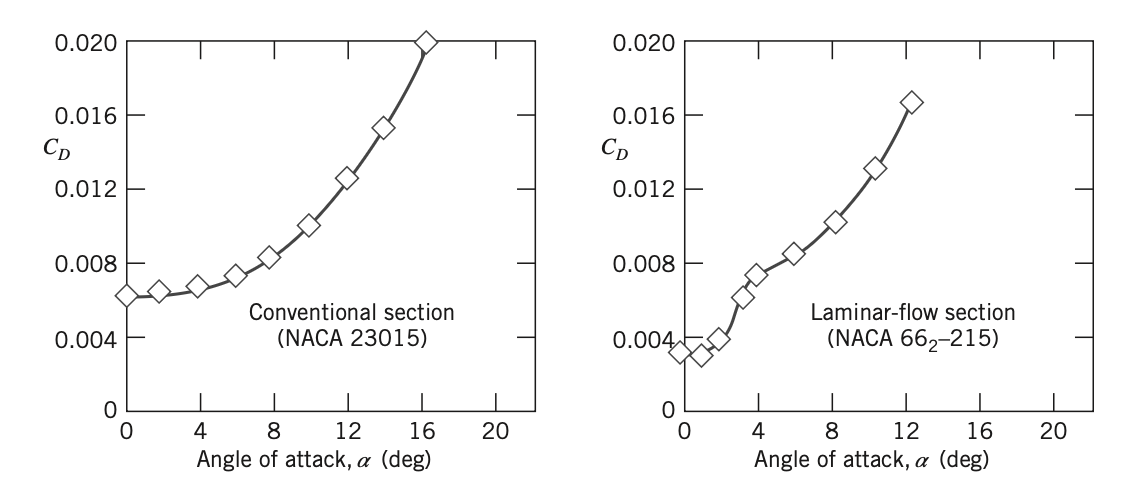
\includegraphics[width=0.7\linewidth]{./figures/f9_17b.png}
  \caption{Drag Coefficient versus angle of attack for two airfoil sections of 15\% thickness ratio at $\mathrm{Re}_c = \num{9e6} $.}
  \label{fig:f9_17b}
\end{figure}

Movement of the minimum pressure point and increase in the adverse pressure gradient are responsible for the sudden increase in $C_D$ for the laminar flow section on \Cref{fig:f9_17b}.
The sudden rise in $C_D$ is caused by transution from laminar to turbulent boundary layer flow on the upper surface.
Aircrafts are designed to cruise in the low drag region.

Because laminar flow sections have very sharp leading edges, all of the described effects are exaggerated, and they will stall at lower AoA's than conventional sections, as shown in \Cref{fig:f9_17a,fig:f9_17b}.

Plots of $C_L$ versus $C_D$ (called \textit{lift-drag polars}) are often used to present airfoil data in compact form. 
In general a high $C_L / C_D$ ratio is the goal for maximizing lifting ability whilst minimizing drag, at which laminar airfoils excel.

All airfoils are of finite span and therefore have less lift and more drag than their airfoil section data would indicate.
This can be explained by the creation of vortices as depicted on \Cref{fig:f9_20}

\begin{figure} [ht]
  \centering
  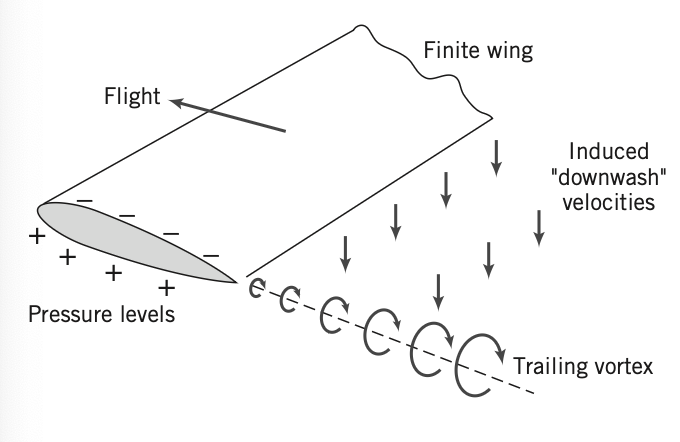
\includegraphics[width=0.5\linewidth]{./figures/f9_20.png}
  \caption{Schematic representation of the trailing vortex system of a finite wing.}
  \label{fig:f9_20}
\end{figure}

Loss of lift and increase in drag caused by these finite-span effects are concentrated near the tip of the wing; hence, a short and stubby wing will experience these effects more severely than a long wing.
We therefore expect the effects to correlate with the wing aspect ratio, defined as
\begin{equation*}
  \mathrm{AR} \equiv \frac{b^2}{A_p}
\end{equation*}
where $A_p$ is the planform area and $b$ is the wingspan.

When the angle of attack of a finite wing is increased, the trailing vortices increase, leading to a loss of lift and increased drag.
The effects of the finite aspect ratio can be characterized as a reduction $\Delta a$ in the effective AoA.
This is theoretically and experimentally determined to be approximately given by
\begin{equation*}
  \Delta \alpha \approx \frac{C_L}{\pi \mathrm{AR}}
.\end{equation*}
The induced drag component of the drag coefficient is
\begin{equation*}
  \Delta C_D \approx C_L \Delta \alpha \approx \frac{C^2_L}{\pi \mathrm{AR}}
.\end{equation*}
This is depicted on \Cref{fig:f9_21}.

\begin{figure} [ht]
  \centering
  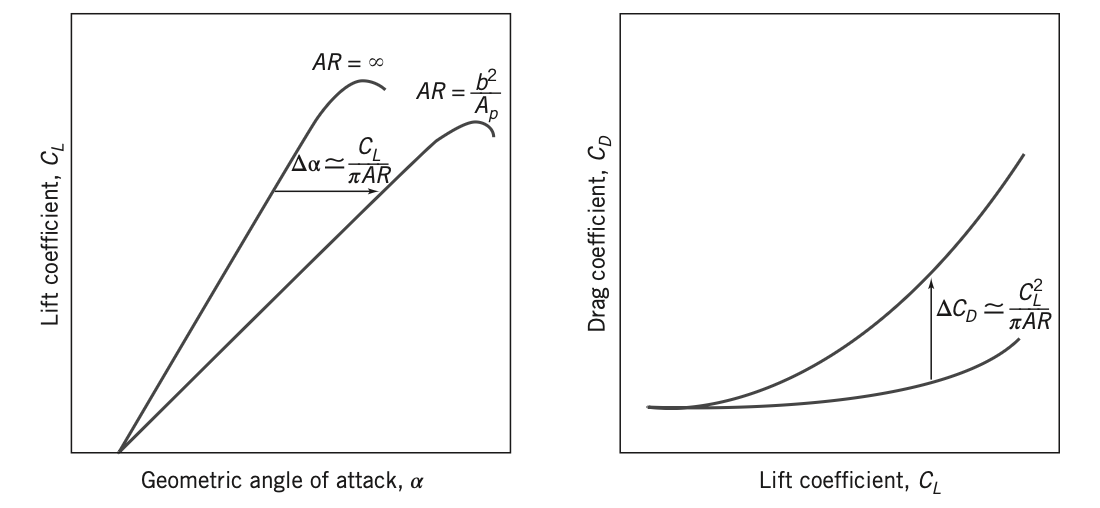
\includegraphics[width=0.6\linewidth]{./figures/f9_21.png}
  \caption{Effect of finite aspect ratio on lift and drag coefficients for a wing.}
  \label{fig:f9_21}
\end{figure}

When written in terms of aspect ratio, the drag of a wing of finite span becomes
\begin{equation*}
  C_D = C_{D, \infty} + C_{D,i} = C_{D, \infty} + \frac{C_L^2}{\pi \mathrm{AR}}
\end{equation*}
where $C_{D, \infty}$ is the section drag coefficient at $C_L$, $C_{D,i}$ is the induced drag coefficient at $C_L$, and $\mathrm{AR}$ is the aspect ratio of the finite-span wing.

The effective aspect ratio of a wing can be improved by adding a winglet to the wing top. These are short, aerodynamically contoured wings set perpendicular to the wing at its tip.
The winglet blocks the flow from crossing between the higher pressure region below the wing tip to the lower pressure region above the top.
This reduces the formation of the trailing vortices which reduces drag on the aircraft.
